\section{Задание 8}

Применить метод Монте-Карло к решению первой краевой задачи для двумерного 
уравнения Лапласа в единичном круге:
\begin{equation} \label{Dirichlet}
    \left\{
    \begin{array}{lcr}
        \Delta u = 0,(x,y) \in D,        \\
        u |_{\delta D }= f(x,y),         \\
        u \in C^2(D), f \in C(\delta D), \\
        D= \{ x,y: x^2 + y^2 \le 1 \}
    \end{array}
    \right.
\end{equation}

Для функции $f(x,y) = x^2 - y^2$ найти аналитическое решение и сравнить с 
полученным по методу Монте-Карло.

\bigskip

Численное решение уравнения Дирихле \eqref{Dirichlet} в круге $D$ можно 
получить таким способом. Для каждой точки $M$ из заданной заранее сетки $N$ 
раз проводится следующая процедура. Сначала строится окружность с центром в 
точке $M$ и максимальным радиусом, таким что эта окружность еще принадлежит 
замыканию $D$. На окружности разыгрывется случайная равномерно распределенная 
точка $M_1$. Если $\rho(M_1, \partial D) < \epsilon$, то процесс 
обрывается и выбирается граничное значение $f(Q^1)$, где $Q^1$~--- ближайшая 
граничная точка, инчаче $M_1$ принимается за следующую точку и процедура 
продолжается. 

После того как такой процесс блуждания производится $N$ раз считается среднее 
арифметическое 
\begin{equation*}
    \frac{f(Q^1) + f(Q^2) + \ldots + f(Q^N)}{N},
\end{equation*}
являющееся приближенным значением искомого решения $u(M)$.

Аналитическим решением \eqref{Dirichlet} для $f(x,y) = x^2 - y^2$ является, 
очевидно, $u~=~x^2~-~y^2$. Сравните аналитическое решение с результатом работы 
описанного выше алгоритма на рис. \ref{dirMC}

\begin{figure}[tbp]
    \centering
    \begin{subfigure}[b]{0.48\textwidth}
        \centering
        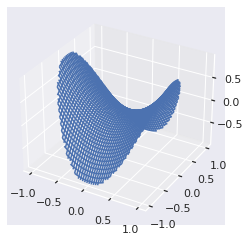
\includegraphics[width=\textwidth]{resources/task8_analytical.png}
        \caption{Аналитическое решение}
    \end{subfigure}
    \hfill
    \begin{subfigure}[b]{0.48\textwidth}
        \centering
        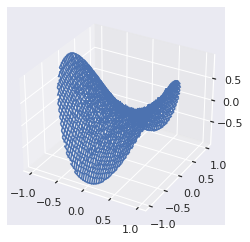
\includegraphics[width=\textwidth]{resources/task8_numerical.png}
        \caption{Численное решение ($N=1000$)}
    \end{subfigure}
    \caption{}
    \label{dirMC}
\end{figure}